%%%%%%%%%%%%%%%%%%%%%%%%%%%%%%%%%%%%%%%%%%%%%%%%%%%%%%%%%%%%%%%%%%%%%%%%
% This is the introduction chapter file.
%%%%%%%%%%%%%%%%%%%%%%%%%%%%%%%%%%%%%%%%%%%%%%%%%%%%%%%%%%%%%%%%%%%%%%%%
%
% Author:   René Widmer
%           Institute for Surgical Technology and Biomechanics ISTB
%           University of Bern
%           rene.widmer@istb.unibe.ch
%
% Date:     10/28/2009
%
%%%%%%%%%%%%%%%%%%%%%%%%%%%%%%%%%%%%%%%%%%%%%%%%%%%%%%%%%%%%%%%%%%%%%%%%

\chapter{Introduction}
\section{Motivation} 
\section{The Liver} 
\subsection{Liver Anatomy}
The human liver overlies the gallbladder, is located in the right upper quadrant of the abdomen and has
different functions. It produces biochemicals necessary for digestion,
synthesizes proteins and detoxifies various metabolites. A human liver wheighs
normally around 1.5 kg, is the heaviest internal organ and the largest gland
of the human body. Two large blood vessels are connected to the liver: the
portal vein and the hepatic artery. Both of them subdivide into small
capillaries called \textit{liver sinusoids} and then lead to the functional
units of the liver known as \textit{lobules}. To refer to the different parts of
the liver, it is subdivided into eight subsegments. Each segment has its own
vascular inflow and outflow.
\begin{figure}[H]
  \centering
 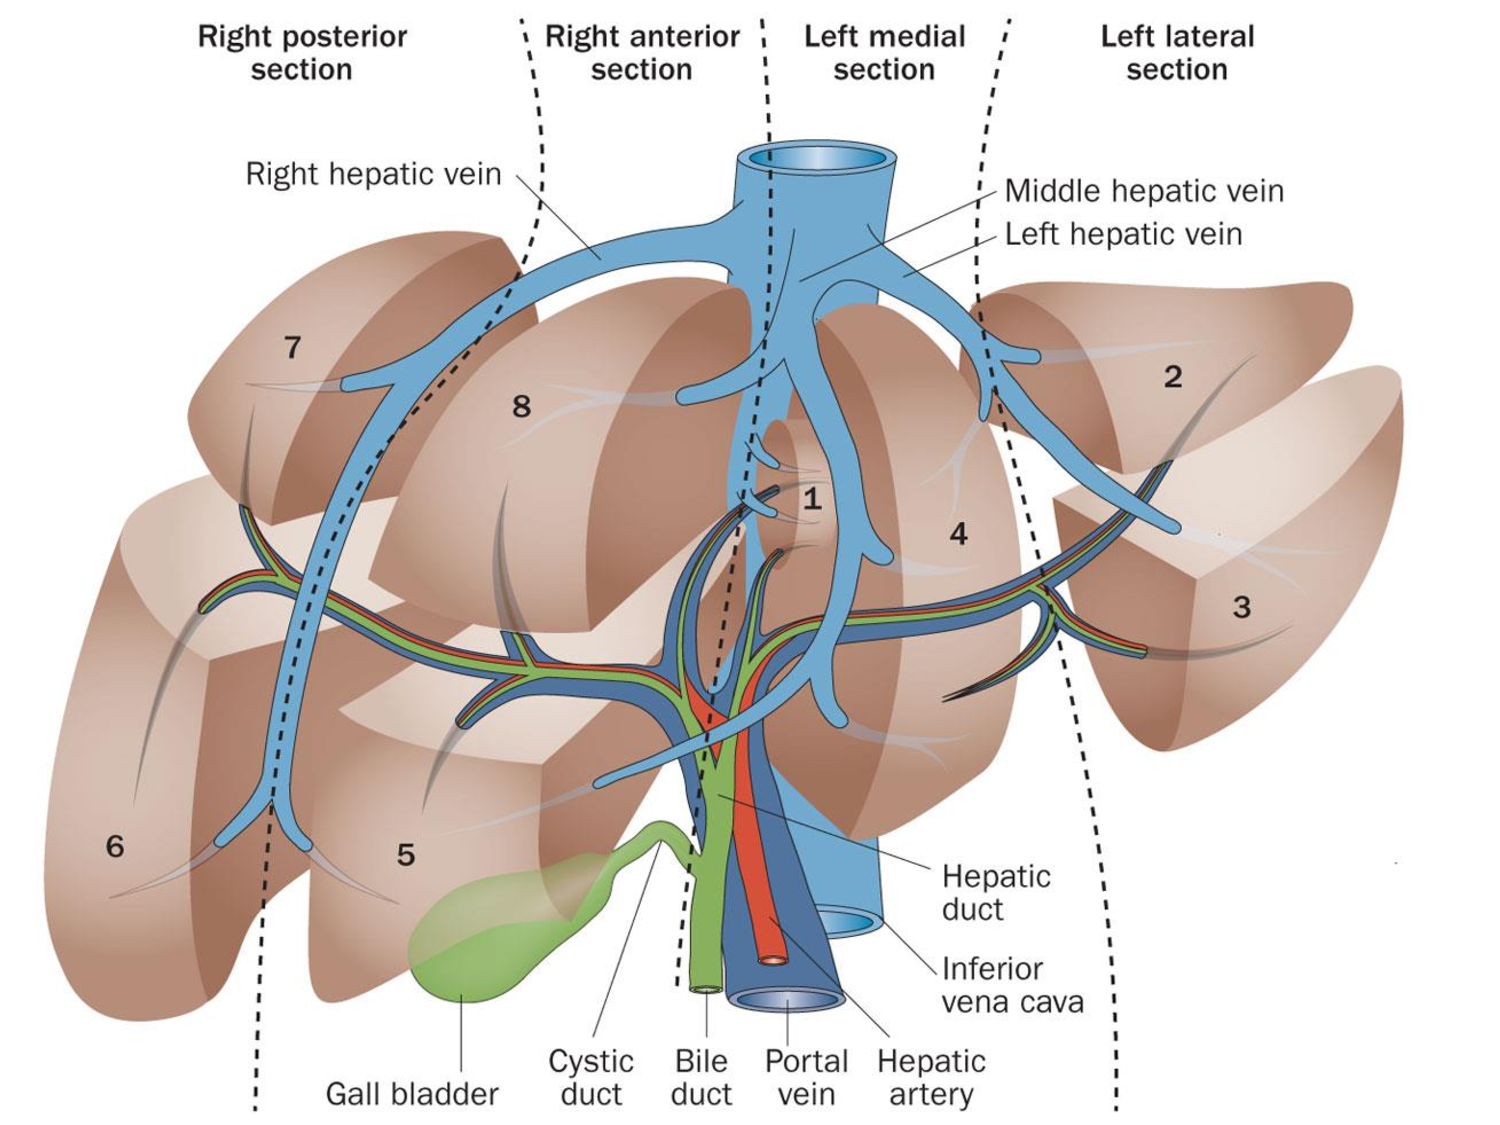
\includegraphics[width=\textwidth]{liverSegments}
  \caption{The liver and its eight Chouinaud segments. In red is the hepatic
    artery which transports blood from the heart a into the liver. In dark blue
    the portal vein, it transports blood from the gut into the liver. All the
    blood leavs the liver through the hepatic veins to the vena cava \cite{siriwardena2014management}.}
  \label{fig:liverSegments}
\end{figure}

\subsection{Liver Cancer}
Liver cancer is cancer that starts in the liver. If the cancer has spread from
elsewhere to the liver, then it is known as liver metastasis. Liver metastasis
are about 20 times more common than primary tumors. One of the reasons for that
is the rich blood supply of the liver which helps the tumors to grow
\cite{mcguire2016world}. Liver cancer patients often have chronic liver diseases
such as cirrhosis, problems of alcohol abuse, and viral hepatitis (B or C)
\cite{galun2015hepatocellular}. The gold standard to treat liver cancer are
surgical resections \cite{lencioni2012local}. The liver tissue can easily regrow, given that after resection there is
enough healthy tissue and blood supply preserved. Alternatively to resections
one can treat liver tumors by local ablation. Both variants treat the tumors
with a safety margin of 10 mm. This safety margin ensures that all tumor cells
are destroyed and to prevent further spread of cancer cells \cite{mahnken2009ct}.
\section{Liver Resections} 
Hepatectomy is the surgical resection (removal of all or part) of the liver.
Liver resections are considered major surgeries and are done under general
anesthesia. Most hepatectomies are done laparoscopicly. However for complicated
cases also open surgeries are done \cite{cherqui2000laparoscopic}. Two
resection techniques can be separated. Anatomical or parenchymal-sparing
resections. This work will concentrate on the latter technique.
\begin{figure}[H]
  \centering
 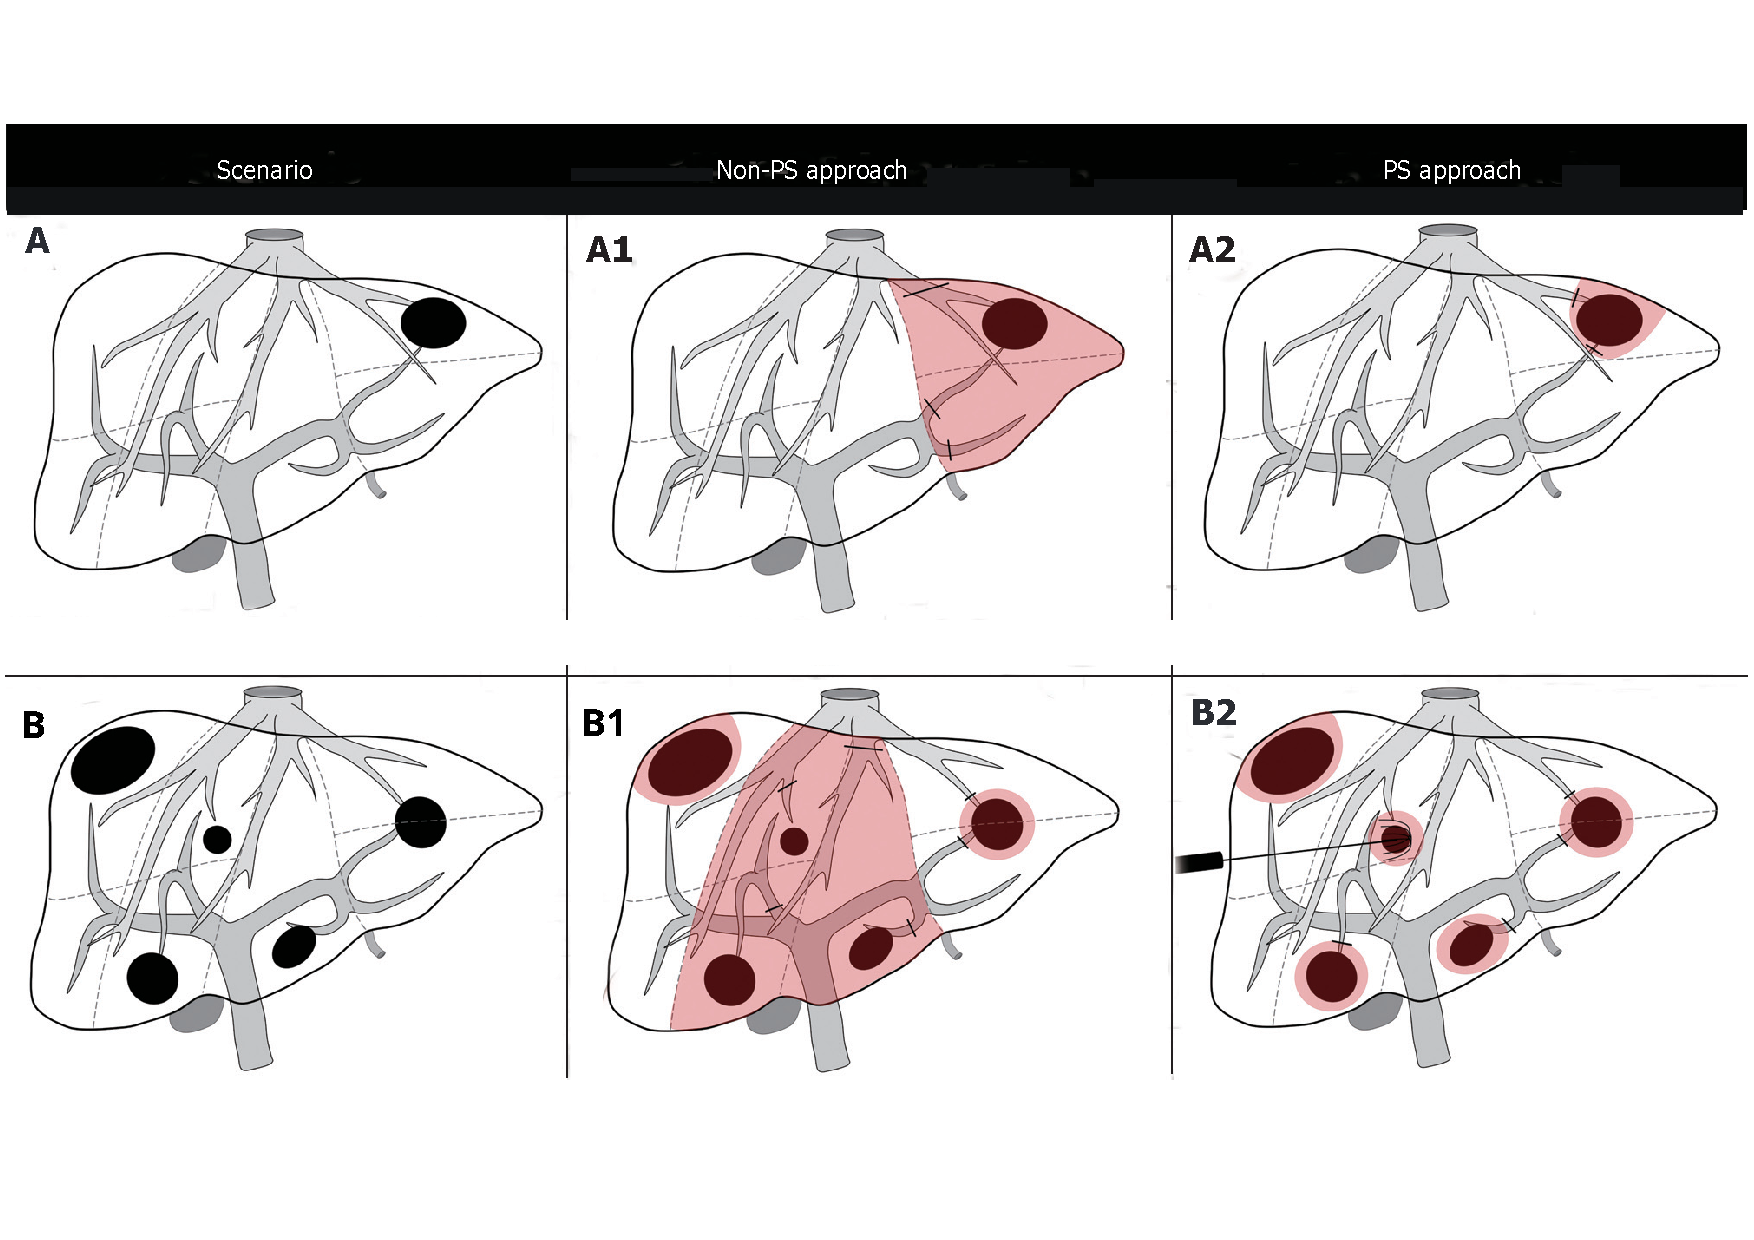
\includegraphics[width=\textwidth]{resectionsPlanning}
  \caption{Two different approaches to resect liver tumors in two different
    situations. The \textit{Scenario} column shows the situation of the
    patient's liver, the \textit{Non-PS approach} column shows how an anatomical
  resection plan would look like and the \textit{PS approach} column shows how a
parenchymal-sparing resection plan would look like \cite{alvarez2016parenchymal}.}
  \label{fig:resectionsPlanning}
\end{figure}

\subsection{Parenchymal-sparing liver surgeries}
\cite{alvarez2016parenchymal}
\section{Objectives} 
Laparoscopic anatomical hepatectomy (LAH)

\endinput
%%% Local Variables:
%%% TeX-master: "MscThesis"
%%% End: